
In dieser Arbeit wurde ein analytisches Modell erstellt, durch welches isolierte Antwortspektren erzeugt werden können, mit denen es möglich ist, Modalanalysen an Gebäudemodellen durchzuführen, ohne den Isolator im Gebäudemodell zu erfassen.
Die isolierten Antwortspektren wurden mit dem hier erarbeiteten Modell aus den Antwortspektren gemäß Eurocode 8 abgeleitet.
Dies hat den Vorteil, dass die Antwortspektren nach bereits etablierten Verfahren für den individuellen Gebäudestandort ermittelt werden können.
Das Modell erspart dem Anwender ebenfalls die eventuell komplexe Modellierung des Gebäudeisolators, da das Verhalten des Isolators im isolierten Antwortspektrum abgebildet ist.
Es ist folglich möglich, Verfahren wie die Modalanalyse oder das vereinfachte Antwortspektrenverfahren unter Verwendung des isolierten Antwortspektrums durchzuführen.

Um das Verhalten eines Isolatortyps im Modell abzubilden, wurden in dieser Arbeit ausschließlich Gleitpendelisolatoren betrachtet.
Gute Isolationseigenschaften werden erzielt, wenn die Steifigkeit des Isolators deutlich kleiner ist als die der aufgehenden Struktur und die Masse direkt über dem Isolator möglichst groß ist.
Die Rückstell- und Reibungskraft ist bei Gleitpendelisolatoren proportional zu ihrer effektiven Steifigkeit.
Die Dämpfung wird in linearer Näherung über die Hystereseschleife und die effektive Steifigkeit berechnet.

Um die Ergebnisse des isolierten Antwortspektrums abschätzen zu können, wurden zunächst Näherungen mithilfe des Modells des effektiven Einmassenschwingers berechnet.
Das isolierte Antwortspektrum wurde dabei zunächst mit einem vereinfachten Verfahren berechnet. Dieses Verfahren lieferte jedoch Werte auf der unsicheren Seite, weshalb ein weiterer Ansatz untersucht wurde.
Dieser zweite Ansatz basiert auf der Berechnung der Transmissibilität, um die Übertragung von Schwingungen aus Fußpunktanregungen auf die aufgehende Struktur via des Isolators zu bestimmen.
Bei diesem  Verfahren ist es zudem möglich, unterschiedliche Dämpfungswerte für Struktur und Isolator anzunehmen.
Im Verlauf dieser Arbeit wurden daher auch verschiedene Dämpfungsmodelle untersucht.

Die Korrektheit des Ableitungsverfahrens und der Dämpfungsmodelle wurde nachfolgend durch vergleichende Beispielrechnungen verifiziert.
Die Ergebnisse wurden mit den Ergebnissen einer numerischen Zeitschrittberechnung und denen des vereinfachten Verfahrens verglichen.
Bei den Vergleichen zeigte sich, dass das Transmissibilitätsverfahren Werte erzeugt, die auf der sicheren Seite liegen und den qualitativen Verlauf der Spektralbeschleunigungen aus den Zeitschrittberechnungen besser abbilden konnte.

Mit einer Modalanalyse wurde weiterhin gezeigt, dass das isolierte Antwortspektrum dazu verwendet werden kann, das Verhalten des Isolators abzubilden, ohne dass dieser in dem Gebäudemodell vorhanden sein muss.
Es wurden so statische Ersatzlasten berechnet, mithilfe derer das Gebäude auf Erdbebensicherheit ausgelegt werden kann, ohne dass der Isolator aufwendig in das Gebäudemodell integriert werden muss.

\section{Aussicht}

Es hat sich gezeigt, dass mit Korrekturfaktoren die Ergebnisse noch deutlich verbessert werden könnten.

Bei den Isolatorparametern wird die Auslenkung $D$ als die maximale Auslenkung angegeben. Wie sich in \cite{Isemann} aber gezeigt hat, stellt sich diese nicht immer ein. Die tatsächliche Auslenkung ist auch abhängig von der Einwirkung.
Eine Vorgehensweise könnte es nun sein, die Abweichung zwischen maximaler und tatsächlicher Auslenkung über verschiedene Parametersätze und Erdbeben mittels Zeitschrittverfahren zu betrachten und zu untersuchen, ob ein Korrekturfaktor für die Auslenkung abgeleitet werden kann.

Bei der Betrachtung verschiedener Modelle für die Dämpfungskorrektur $\eta$ am Antwortspektrum wurde deutlich, dass auch hier optimiert werden könnte. Ebenfalls wurde in \cite{Isemann} ein realistischerer Dämpfungskorrekturbeiwert als Mittelwert über die Ergebnisse der Zeitschrittberechnung bestimmt. Auch hier wäre es denkbar zu untersuchen, ob es möglich ist, eine Beziehung zu finden, mit der sich der Dämpfungskorrekturbeiwert anpassen ließe.

\section{Excel-Tabelle zur Berechnung von Isolationsspektren}

Die Berechnung des Isolationsspektrums über die Transmissibilität wurde im Rahmen dieser Arbeit mit dem Ansatz aus \cref{sec:Korrekturansaetze} in einer \emph{Excel}-Tabelle implementiert.

So kann nach Eingabe der Parameter 

\makebox[1cm]{$T_B$}  = Eckperiode $[s]$ \par
\makebox[1cm]{$T_C$}  = Eckperiode $[s]$ \par
\makebox[1cm]{$T_D$}  = Eckperiode $[s]$ \par
\makebox[1cm]{$S$}    = Bodenparameter $[-]$ \par
\makebox[1cm]{$a_g$}  = Bodenbeschleunigung $[m/s^2]$ \par

\pagebreak

das Antwortspektrum (für $5 \%$ Dämpfung, $\eta = 1.0$) ermittelt und graphisch dargestellt werden.
Mit der Angabe der beschreibenden Werte des Isolators

\makebox[1cm]{$D$}    = Auslenkung $[m]$ \par
\makebox[1cm]{$R$}    = Radius der Gleitfläche $[m]$ \par
\makebox[1cm]{$\mu$}  = Reibungskoeffizient $[-]$ \par

werden dessen effektive Dämpfung $\xi_2$, Steifigkeit $k_2$ und Periode $T_2$ berechnet. Es fehlen noch die Werte des Bauwerks

\makebox[1cm]{$m_1$}  = Masse der aufgehenden Struktur $[t]$ \par
\makebox[1cm]{$m_2$}  = Masse direkt über dem Isolator $[t]$ \par
\makebox[1cm]{$\xi_1$} = Dämpfung der aufgehenden Struktur $[-]$ \par

und das Isolationsspektrum wird ausgegeben und graphisch dargestellt.

\begin{figure}[H]
    \centering
    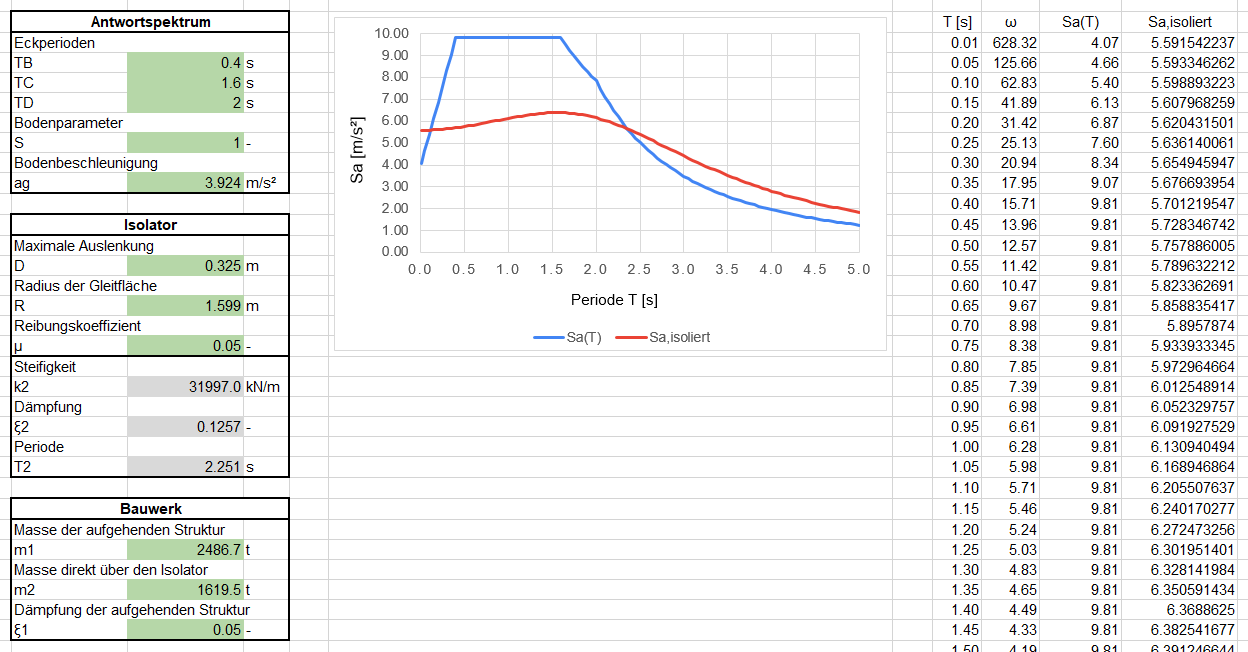
\includegraphics[width=1.0\textwidth]{Excel.png}
    \caption{Excel Tabelle zur Berechnung von Isolationsspektren}
    \label{fig:excel}
\end{figure}


\pagebreak